\chapter{Analysis}
	[TODO:felvezets]
	Nowadays almost every new car has some level of automated driving assistant feature.
	\section{Model of a self driving car}
		So the task is to find a model of an autonomous driver. The key observation is that an self driven car can be modeled with the same model as used before. The only difference relies on IDM and MOBIL parameters. So the task is to find proper parameters for the model that can be used for autonomous driver simulation.
	
		There are three main components representing human behavior built in the model currently. The first one is the attention for driving. An autonomous driver always paying attention to the road. The other component is that a self driving car can always pay attention to both longitudinal and transversal motions. They are not limited to longitudinal motion attention when they have a higher acceleration or deceleration value. The last but not least component that it can have more favorable IDM and MOBIL parameters than most of the non self driving cars. E.g. an autonomous driver will always accelerate with the greatest possible value which is comfortable, they would not change lanes if the advantage they would get be marginal however would put others significantly worst position.
	\section{Self driving car variations}
		To test the effect of autonomous drivers in traffic, the same red traffic light situation was implemented. However in this case one of the driver's parameters have been substituted with an autonomous driver parameters. The most representative figure of the result of this task is where the count of cars passed the target line - 100 meters - is illustrated as a function of time. 
		\subsection{Effect of 1 self-driving car}
		Cars one by one have been exchanged and then simulated with the reaming cars. So a total of ten simulations were run. The result can be seen on Figure \ref{fig:vehicle_density}.
		\begin{figure}
			\centering
			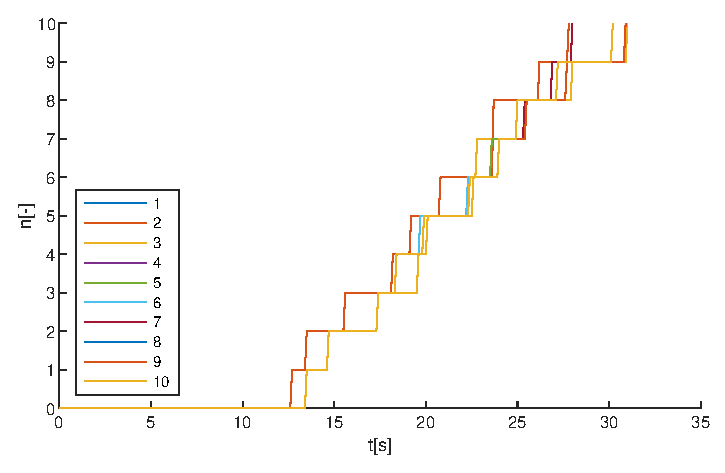
\includegraphics[width=0.75\textwidth]{eemobil/vehicle_density}
			\caption{Number of vehicles passes the target line with one self-driving car}
			\label{fig:vehicle_density}
		\end{figure}

		As Figure \ref{fig:vehicle_density} shows the first car reaches the target line in ~13 seconds. The interesting part is at the top right corner of the figure, where it can be seen that depending on which car has been exchanged the overall elapsed time can change up to 10 \%. The minimum, maximum, average and standard deviation values can be found in Table \ref{tab:vehicle_density_minmaxavg_case1}.
		\begin{table}
			\begin{center}
				\begin{tabular}{ |c|c|c|c|}
					\hline
					\vehicledensitytable{1}
					\hline
				\end{tabular}
			\end{center}
			\caption{Time until the last car has reached the target line. 1 autonomous car}
			\label{tab:vehicle_density_minmaxavg_case1}
		\end{table}
		
		In the hope of a better figure the same simulation results are shown on Figure \ref{fig:vehicle_density_avg} with averaged representation. It is slightly better than previously.
		
		\begin{figure}
			\centering
			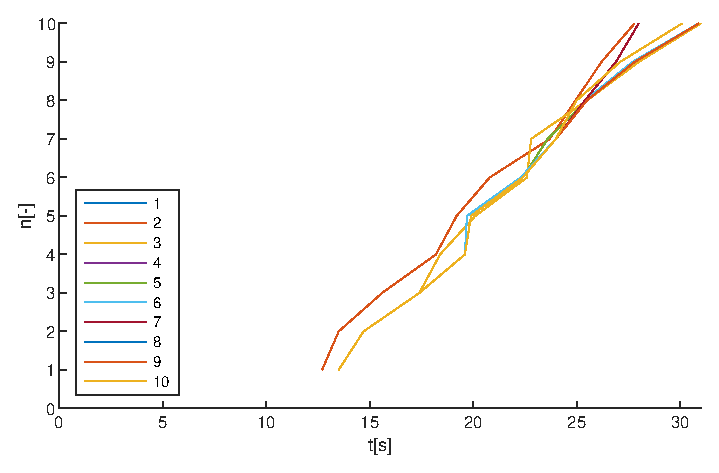
\includegraphics[width=0.75\textwidth]{eemobil/vehicle_density_avg}
			\caption{Number of vehicles passes the target line with one self-driving car}
			\label{fig:vehicle_density_avg}
		\end{figure}
		
		These simulations were run with only one self-driving car but in different positions. It can be seen that one autonomous driver could make the traffic faster. Based on the position of that one car most of the time it will decrease the overall duration.
		\subsection{Effect of 2 self-driving cars}
		Let us try the same simulation but this time run it exchanging two drivers to autonomous driver and see how the situation will improve. The total number of simulation was 45. All unique combinations were simulated. Figure \ref{fig:vehicle_density_case_2} and Table \ref{tab:vehicle_density_minmaxavg_case2} show the result.
		It can be seen that the minimum duration has decreased further.
		\begin{table}
			\begin{center}
				\begin{tabular}{ |c|c|c|c|}
					\hline
					\vehicledensitytable{2}
					\hline
				\end{tabular}
			\end{center}
			\caption{Time until the last car has reached the target line. Two autonomous car}
			\label{tab:vehicle_density_minmaxavg_case2}
		\end{table}
		\begin{figure}
			\centering
			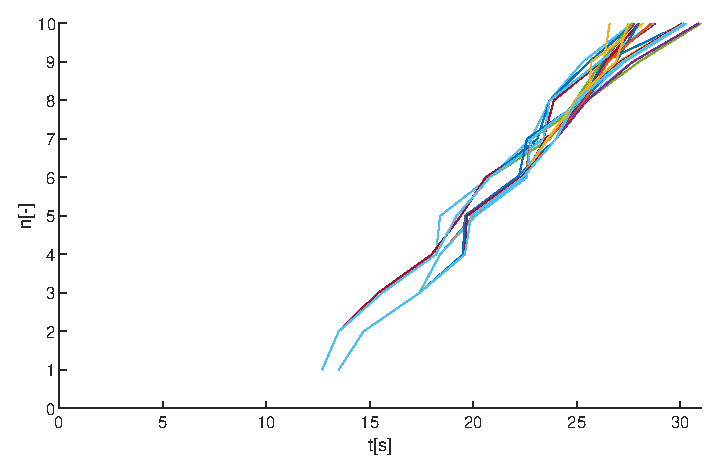
\includegraphics[width=0.75\textwidth]{eemobil/vehicle_density_case_2}
			\caption{Number of vehicles passes the target line with two self-driving cars}
			\label{fig:vehicle_density_case_2}
		\end{figure}

		\subsection{Effect of 3 self-driving cars}
		The same simulations were run with three self-driving cars as well. The total number of 120 unique combinations were simulated. Figure \ref{fig:vehicle_density_case_2} and Table \ref{tab:vehicle_density_minmaxavg_case2} show the result.
		\begin{table}
			\begin{center}
				\begin{tabular}{ |c|c|c|c|}
					\hline
					\vehicledensitytable{3}
					\hline
				\end{tabular}
			\end{center}
			\caption{Time until the last car has reached the target line. Three autonomous car}
			\label{tab:vehicle_density_minmaxavg_case3}
		\end{table}
		\begin{figure}
			\centering
			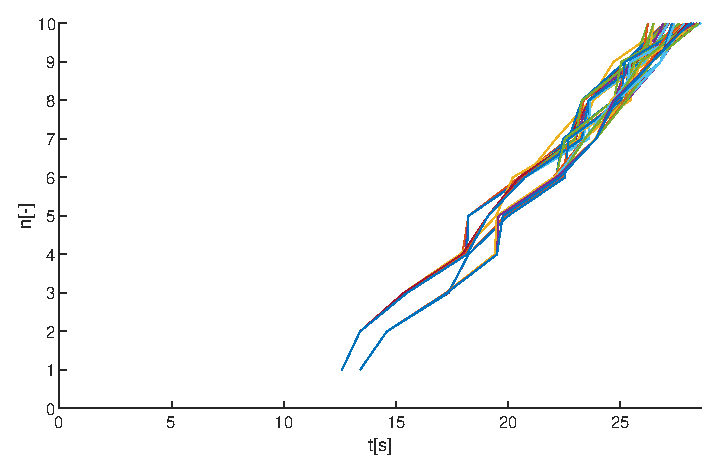
\includegraphics[width=0.75\textwidth]{eemobil/vehicle_density_case_3}
			\caption{Number of vehicles passes the target line with three self-driving cars}
			\label{fig:vehicle_density_case_3}
		\end{figure}
		\subsection{Analyzing all of the combinations}
		As seen in the previous examples the more self-driving vehicles in the traffic the better. So let us investigate all possible combinations to see what is the connection between the time and the number of self-driving cars. The expectation is that until a certain point the connection is almost linear but after that point self driving cars cannot make traffic situation better.
		So all the possible combinations were simulated from only one exchanged car until all the ten cars exchanged. The total number of simulations were 1023.
		\begin{figure}
			\centering
			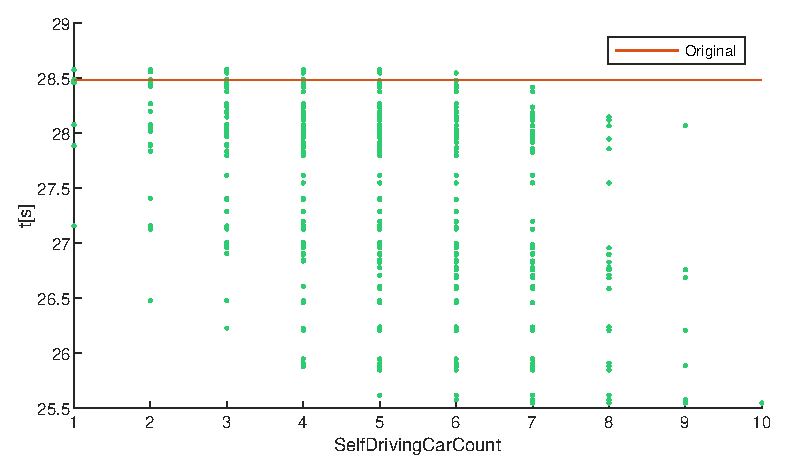
\includegraphics[width=0.8\textwidth]{eemobil/variations_nosize}
			\caption{Time variation of autonomous drivers}
			\label{fig:self_variations_nosize}
		\end{figure}

		The result can be seen on Figure \ref{fig:self_variations_nosize}. The horizontal axis represents how many car has been exchanged. The vertical axis shows the duration of the simulation. Unfortunately most of the points are in the same place - because of the time step - so the figure could be a little bit misleading. To make it more expressive the plot has been modified to show a larger dot where there are more simulation results and smaller where there are just a few. The result of this modification can be seen on Figure \ref{fig:self_variations}.
		\begin{figure}
			\centering
			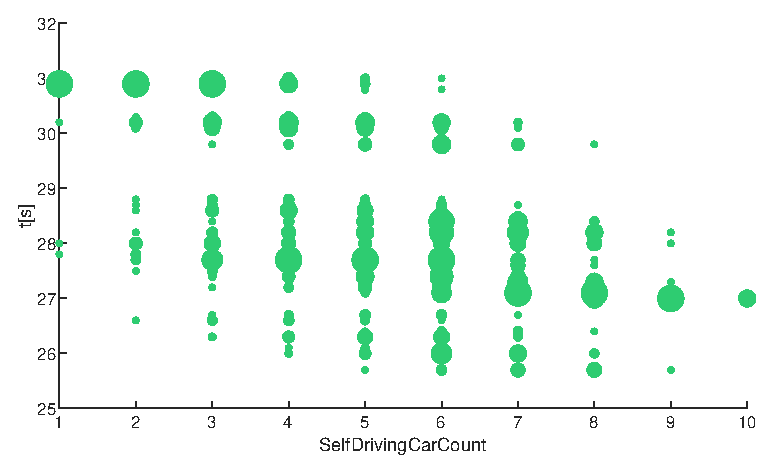
\includegraphics[width=0.8\textwidth]{eemobil/variations}
			\caption{Time variation of autonomous drivers}
			\label{fig:self_variations}
		\end{figure}
		
		On Figure \ref{fig:self_variations} there are multiple 
		\begin{figure}
			\centering
			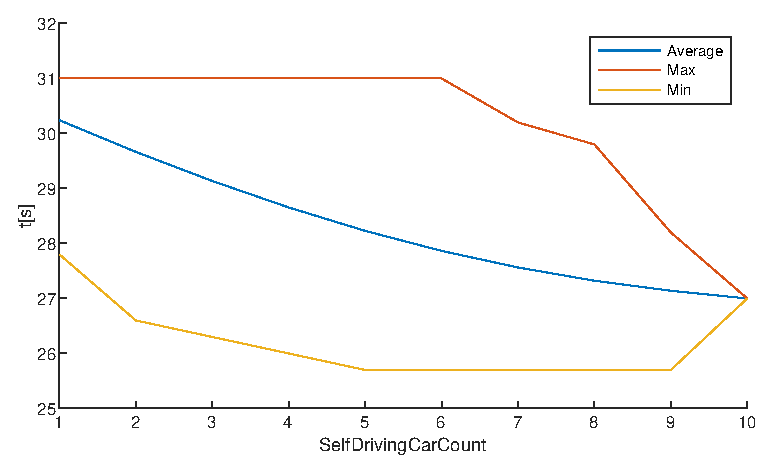
\includegraphics[width=0.8\textwidth]{eemobil/variations_avgminmax}
			\caption{Average, minimum and maximum of elapsed time.}
			\label{fig:self_variations_avgminmax}
		\end{figure}
		\begin{figure}
			\centering
			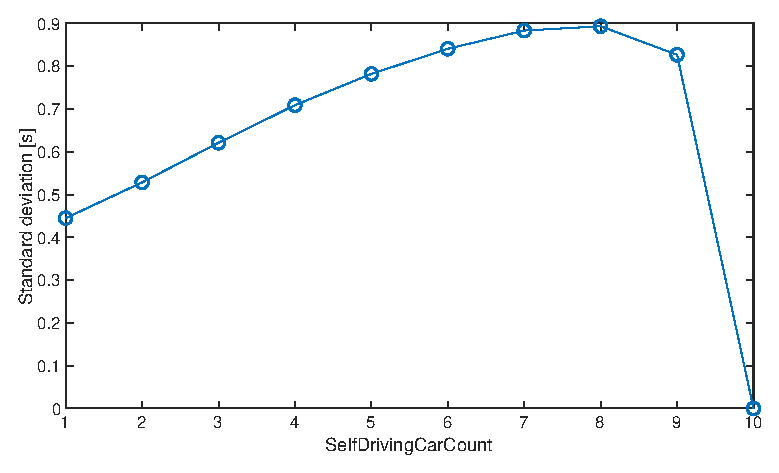
\includegraphics[width=0.8\textwidth]{eemobil/variations_std}
			\caption{Standard deviation of elapsed time}
			\label{fig:self_variations_std}
		\end{figure}
